\documentclass[twocolumn,11pt]{article}
\usepackage{fullpage}
\usepackage{hyperref}
\usepackage{amsmath}
\usepackage{amssymb}
\usepackage{amsthm}
\usepackage{fancybox}
\usepackage{graphicx}
\usepackage{caption}
\usepackage{subcaption}
\usepackage{float}
\usepackage{natbib}
\bibliographystyle{abbrv}

\begin{document}

\title{Pandora: microbial characterization of tumor tissue from whole transcriptome sequencing}

\author{Sakellarios Zairis$^*$, Francesco Abate$^*$, Oliver Elliott, and Raul Rabadan\\
\\
Department of Systems Biology, Columbia University}
\maketitle


%%%%%%%%%%%%%%%%%%%%%%%%%%%%%%%%%%%%%%%%%%%%%%%%%%%%%%%%%%%%%%%%%%%%%%%%%%%%%%%%%%%%%%%%%%%%%%%%%%%%
%%%%%%%%%%%%%%%%%%%%%%%%%%%%%%%%%%%%%%%%%%%%%%%%%%%%%%%%%%%%%%%%%%%%%%%%%%%%%%%%%%%%%%%%%%%%%%%%%%%%

\begin{abstract}

Whole transcriptome sequencing (RNAseq) of human tissue has traditionally been used for gene expression profiling.
The compartment of transcripts not deriving from the human genome, however, offers a limited window into host-microbe interactions and local tissue conditions.
Microbial detection from RNAseq typically follows the strategy of \textit{in silico} host subtraction, followed by a combination of database local alignment and \textit{de novo} assembly.
One step beyond detection, however, lie the issues of annotating the functional significance of non-human transcripts and quantifying host-microbe interactions.
We implement an open-source pipeline, for nominating microbial taxa whose concentration in a series of tissue samples carries an interpretable correlate in the host expression profile.
Active viral replication detected in tumor samples can point to local suppression of immune surveillance, or identify infection with a known oncovirus.
Cellular microbe populations nominated by Pandora can indicate global immunocompromise or inform anti-microbial regimens, while bacterial oxygen preferences can help identify hypoxia in tumor samples prior to a therapy whose efficacy is a strong function of oxygen tension. 

\end{abstract}

%%%%%%%%%%%%%%%%%%%%%%%%%%%%%%%%%%%%%%%%%%%%%%%%%%%%%%%%%%%%%%%%%%%%%%%%%%%%%%%%%%%%%%%%%%%%%%%%%%%%
%%%%%%%%%%%%%%%%%%%%%%%%%%%%%%%%%%%%%%%%%%%%%%%%%%%%%%%%%%%%%%%%%%%%%%%%%%%%%%%%%%%%%%%%%%%%%%%%%%%%

\section*{Introduction}

In the clinical setting, capture libraries (mRNA, exome) are far more prevalent than shotgun sequencing, since questions of pathogenesis are often more directly answered by focusing on the the human coding genome.
This limits the opportunity for microbial profiling of clinical sequencing samples, but does not extinguish it entirely.
[sentence about the increasing recognition of the microbial contribution to cancer.]


For over half a century it has been known that bacterial spores from obligate anaerobes can migrate to and germinate within hypoxic regions of mammalian tumors.~\cite{malmgren1955localization}
We 


%%%%%%%%%%%%%%%%%%%%%%%%%%%%%%%%%%%%%%%%%%%%%%%%%%%%%%%%%%%%%%%%%%%%%%%%%%%%%%%%%%%%%%%%%%%%%%%%%%%%
%%%%%%%%%%%%%%%%%%%%%%%%%%%%%%%%%%%%%%%%%%%%%%%%%%%%%%%%%%%%%%%%%%%%%%%%%%%%%%%%%%%%%%%%%%%%%%%%%%%%

\section*{Methods}

We follow a strategy of ``digital transcriptome subtraction,'' first successfully deployed in the discovery of Merkel cell polyomavirus.~\cite{feng2008clonal}
The overall Pandora workflow, along with some basic calibration can be seen in Figure \ref{fig:pipeline}

\begin{figure}
    \begin{subfigure}{0.5\textwidth}
    \centering
    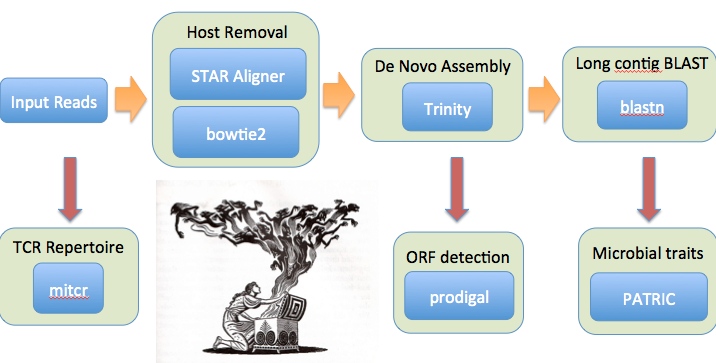
\includegraphics[width=2.5in]{fig/schematic.png}
    \caption{caption goes here.}
    \end{subfigure}
    
    \begin{subfigure}{0.5\textwidth}
    \centering
    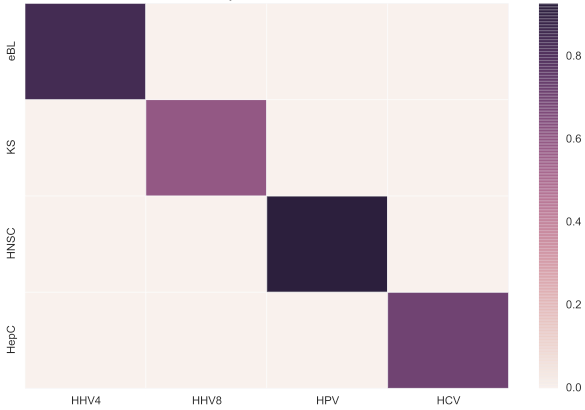
\includegraphics[width=2.5in]{fig/sensitivity_panel.png}
    \caption{caption goes here.}
    \end{subfigure}

    \caption{overall caption.}
    \label{fig:pipeline}
\end{figure}

%%%%%%%%%%%%%%%%%%%%%%%%%%%%%%%%%%%%%%%%%%%%%%%%%%%%%%%%%%%%%%%%%%%%%%%%%%%%%%%%%%%%%%%%%%%%%%%%%%%%
%%%%%%%%%%%%%%%%%%%%%%%%%%%%%%%%%%%%%%%%%%%%%%%%%%%%%%%%%%%%%%%%%%%%%%%%%%%%%%%%%%%%%%%%%%%%%%%%%%%%

\section*{Results}

The ideal data set would be total RNA libraries, with matched normal samples, so we investigated the publicly available data accompanying \cite{warren2013co}.
We also wish to extend the analysis to the mRNA capture libraries of TCGA.
An example of an old result in alcoholic liver disease can be seen in Figure \ref{fig:alcoholic}

\begin{figure}
    \begin{subfigure}{0.5\textwidth}
    \centering
    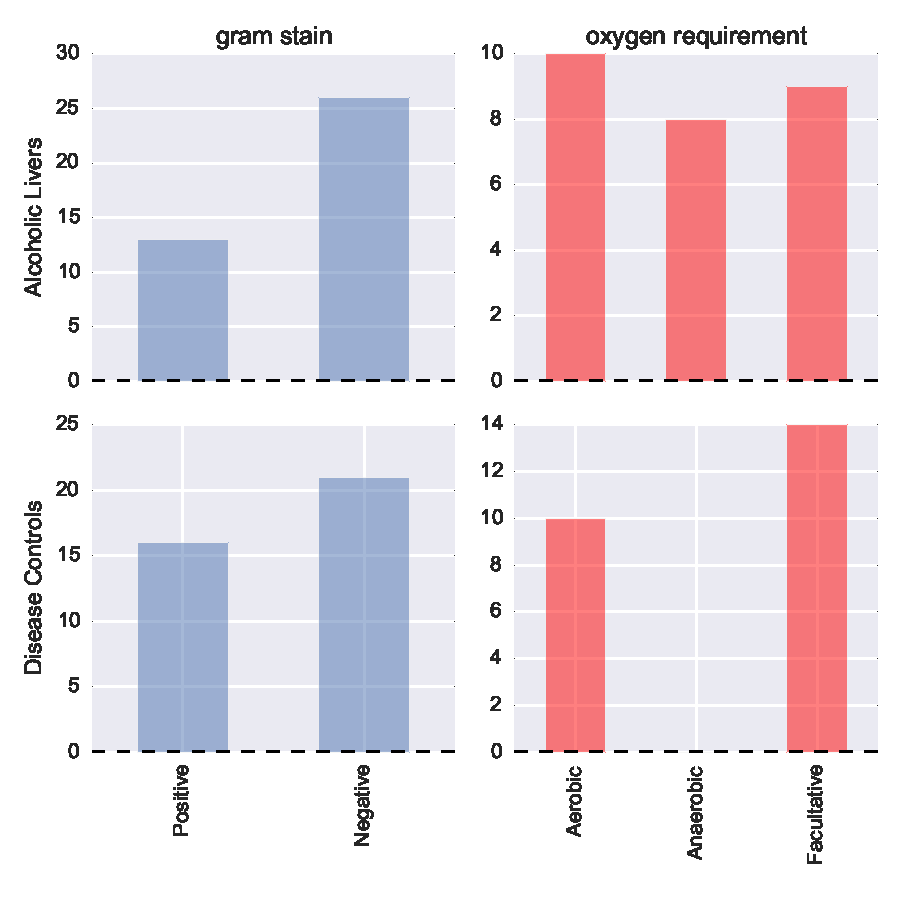
\includegraphics[width=2.5in]{fig/liver_patric.pdf}
    \caption{caption goes here.}
    \end{subfigure}
    
    \begin{subfigure}{0.5\textwidth}
    \centering
    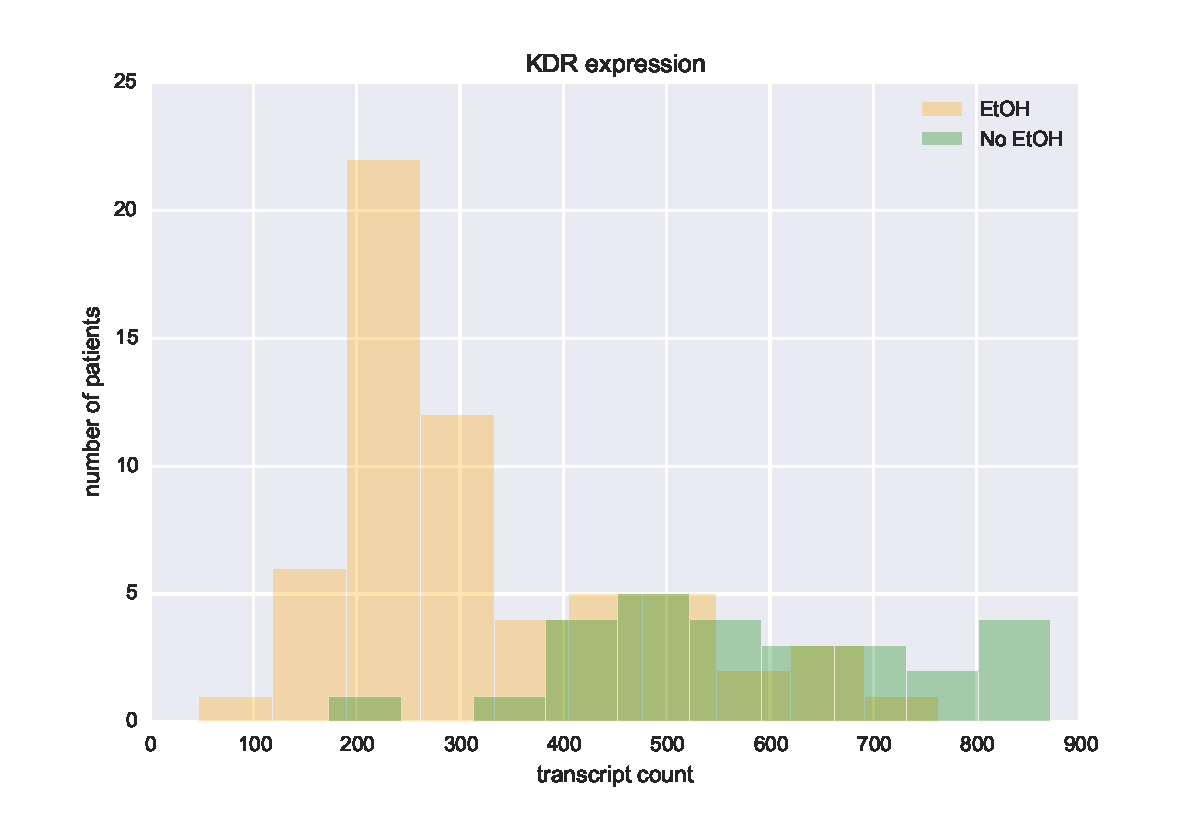
\includegraphics[width=2.5in]{fig/liver_KDR.pdf}
    \caption{caption goes here.}
    \end{subfigure}

    \caption{overall caption.}
    \label{fig:alcoholic}
\end{figure}

%%%%%%%%%%%%%%%%%%%%%%%%%%%%%%%%%%%%%%%%%%%%%%%%%%%%%%%%%%%%%%%%%%%%%%%%%%%%%%%%%%%%%%%%%%%%%%%%%%%%
%%%%%%%%%%%%%%%%%%%%%%%%%%%%%%%%%%%%%%%%%%%%%%%%%%%%%%%%%%%%%%%%%%%%%%%%%%%%%%%%%%%%%%%%%%%%%%%%%%%%

\section*{Discussion}

State the result here.

%%%%%%%%%%%%%%%%%%%%%%%%%%%%%%%%%%%%%%%%%%%%%%%%%%%%%%%%%%%%%%%%%%%%%%%%%%%%%%%%%%%%%%%%%%%%%%%%%%%%
%%%%%%%%%%%%%%%%%%%%%%%%%%%%%%%%%%%%%%%%%%%%%%%%%%%%%%%%%%%%%%%%%%%%%%%%%%%%%%%%%%%%%%%%%%%%%%%%%%%%

\subsection*{Acknowledgments}

This work is supported by a TL1 personalized medicine fellowship (5TL1TR000082), and NIH grants (R01 CA179044, R01CA185486, R01GM117591, U54 CA193313).

%%%%%%%%%%%%%%%%%%%%%%%%%%%%%%%%%%%%%%%%%%%%%%%%%%%%%%%%%%%%%%%%%%%%%%%%%%%%%%%%%%%%%%%%%%%%%%%%%%%%
%%%%%%%%%%%%%%%%%%%%%%%%%%%%%%%%%%%%%%%%%%%%%%%%%%%%%%%%%%%%%%%%%%%%%%%%%%%%%%%%%%%%%%%%%%%%%%%%%%%%

\bibliography{refs}

\end{document}
